\documentclass{book}
\usepackage[english]{babel}
\usepackage[utf8]{inputenc}
\usepackage{float}
\usepackage{graphicx}
\usepackage{subfig}
\usepackage{hyperref}
\usepackage{wrapfig}
\usepackage{listings}
\usepackage{fullpage}
\usepackage{caption}
\usepackage{cite}

\begin{document}

\begin{titlepage}
   \begin{center}
       \vspace*{1cm}

       \textbf{Electricity Bill Price Prediction}

       \vspace{0.5cm}
       Analysis based on European Union integration level
            
       \vspace{1.5cm}
       \textbf{Francesco Cabras}
       \vfill
       
\includegraphics[width=0.4\textwidth]{Images/unitn.png}            
       \vspace{0.8cm}
            
       Dipartimento di Matematica\\
       Università degli Studi di Trento\\
       Italy\\
       \today
            
   \end{center}
\end{titlepage}

\chapter*{Introduction}

Electricity bills are among the most important expenses for families around the world, at least for the lucky households that have access to it. In distinct countries the price of electricity of course is different, and it is not only always easy to acknowledge which are the reasons behind these gaps. One could think that the key factor is in the supply: how much it costs to actually source energy, getting electricity and especially distribute it among households. In recent years many countries around the world have gone through liberalization of their electricity markets: the result is that consumers can choose among different suppliers, and may decide to modify the profile of their demand to reduce their costs \cite{867149}. This means that the demand of electricity has become more elastic. Another trend that has gone through in recent years has been the increase in the renewable sources of energy. To measure the effect of such changes on the price of the good is the main aim of this document. The first idea is to have a look at the amount spent by households aroung the world for their electricity bills.  In \textit{Figure 1} the countries are colored on the basis of the price of electricity, measured in US dollars per kWh \footnote{World Bank data, 2020}.

\bigskip
\begin{figure}[H]
\begin{center}
\captionsetup{justification=centering}
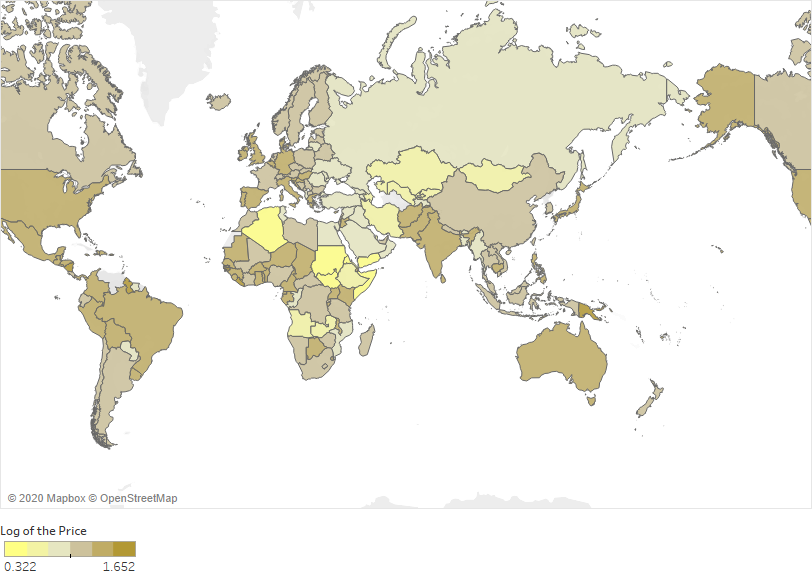
\includegraphics[width=0.9\textwidth]{Images/world2020.png}
\caption{The more expensive electricity is, the more intense the red color. }
\end{center}
\end{figure}
\bigskip

The more intense the red color, the more expensive electricity is. Interestingly, the country which appears as the most intensely red-colored is among the ones that has the easiest access to resources for getting electricity: \textbf{Venezuela}.The reason behind this finding is that in recent years this country has been suffering from exceptional inflation: the take-home message, however, is that the political and macro-economical frameworks are extremely important for the final price of this good.\\

Apart from South America, also in Africa some results are quite interesting: looking at the pale color of countries like South Sudan or Somalia, which are among the poorest in the world, the reader may think that to wealthier country consistently should correspond higher electricity price, given that there is no sky-high inflation. If however, for instance, bordering countries as Algeria and Niger countries are considered, this simple hypothesis does not work: the former has an electricity price of 2.1 dollars per kWh and a gdp per capita of 4,114.72 dollars. In the latter, instead, electricity price corresponds to 21.3 dollars per kWh (10 times with respect to Algeria) but the gdp is merely 413.98 dollars (almost one tenth with respect to Algeria) \footnote{World Bank data, 2020}. Since inflation is not really a problem in Niger, this is a hint that the link between economic development and electricity price is not that elementary.

\section*{European Union Electricity Market}

Electricity is not an easily tradable product, as it needs hundreds of  legal rules and technical standards to be agreed upon before it can become freely marketable. Electric power is, after all, not more than a flow of electrons inside metallic wires of a massive, interconnected network. That is the reason why, for decades, electricity was considered to be an "anti-market" product, best suited to non-competitive markets like natural monopolies. \cite{glachant2014eu} Furthermore, the particular characteristics of electricity, such as non-storability and the continuous balance between demand and supply, supported the State intervention. The fact that this market is inclined to be a monopoly resulted in efficiencies, where State subsidies have been the rule to maintain a stable industry. \cite{domanico2007concentration} Nevertheless, there is one region in the world that has tried to overcome these "anti-market" barriers to create an extremely vast electricity market. That region is identifiable as the European Union. \\

The European Union because is a unique case of a large extended market in which member countries can exchange goods.  Liberalization of the economic markets and convergence are two of the main objectives in the Union. In particular, European electricity market liberalization represents the world's most large-scale cross-jurisdiction reform of the electricity sector involving integration of national markets. To reach such a big achievement took several years of time, and there are specific reasons why this process took so long:

\begin{itemize}

\item The objective of this project is to open up national monopolies’ market spaces to foreigners, which of course is a radical
project that inevitably leaves some parties unsatisfied.  One of the risks of market concentration is that big incumbents try to build
barriers in order to maintain their position and to foreclose the entrance of more efficient market actors. \cite{ringel2003liberalising}

\item In the last 25 years there has been no wave of disruptive technological innovation to challenge the incumbent energy
giants.

\item the national arrangements that had been developed between industry players and public authorities could not be easily merged at the EU level into a common scheme.
\end{itemize}

Creating a market that is actually free, however, is not an easy matter, and that's why there are still wide differences in the amounts households from different member countries pay for electricity. Although the pace of the liberalization is steady, the integrated European electricity market is yet to be achieved. \\

\subsection*{Taxation}

Taxes account for a sizable share of the final prices consumers pay for energy around the EU and can have a strong impact on consumption patterns, the type of energy consumed and their use. There is disagreement among European countries for much households should pay in their bills, and the consequence is wide differences in tax rates. Belgium, Ireland, Germany and Denmark are the member states where electricity is the most expensive. However, these four countries present different tax rates: Belgium and Ireland citizens pay a high price because electricity is actually expensive excluding taxes and levies while Germany and especially Denmark pay such a high price precisely because of taxes and levies. This behavior is well represented with \textit{Figure 2}, where household electricity prices are plot both including and excluding taxes and levies. Prices are lowest in Bulgaria and Hungary, whose inhabitants pay one third of the amounts Danish citizens pay in their bills. 

\bigskip
\begin{figure}[H]
\begin{center}
\captionsetup{justification=centering}
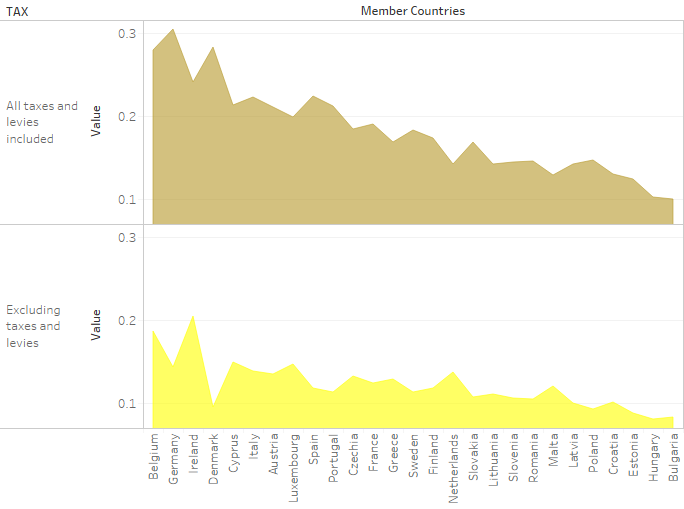
\includegraphics[width=0.9\textwidth]{Images/Taxes.png}
\caption{2019 (second semester) data, electricity prices. }
\end{center}
\end{figure}
\bigskip

The average final price paid by European households is 18.6 cents per KwH including taxes and 12.3 cents per KwH excluding taxes, which make up an average of around 6 cents of taxes per KwH. Over time, also taxes tend to change: in the first semester of 2020 the price paid by European households fell with respect to 2019 by 1.2 cents, while the the electricity price itself decreased only by half a cent. This means that most of the drop was due to a decrease in taxes. \textit{Figure 3} shows how electricity prices for European citizens changed over time, on average.

\bigskip
\begin{figure}[H]
\begin{center}
\captionsetup{justification=centering}
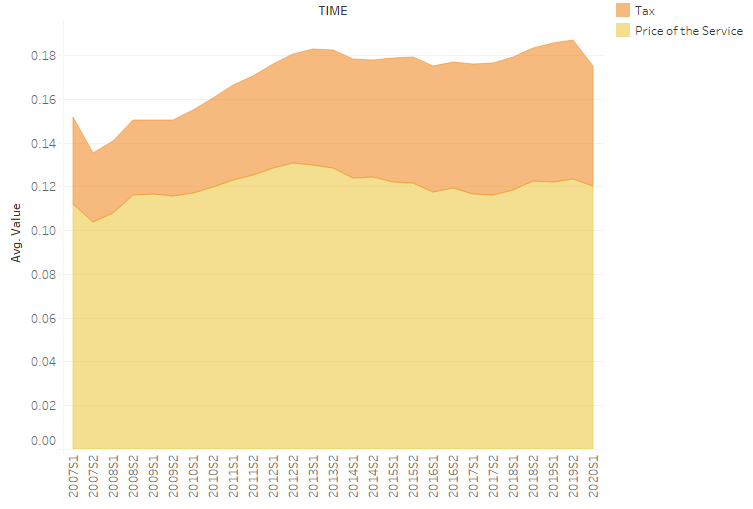
\includegraphics[width=0.9\textwidth]{Images/TaxesTime.png}
\caption{2019 (second semester) data, electricity prices. }
\end{center}
\end{figure}
\bigskip


\subsection*{Concentration}

The directive 2003/54/EC requires that all non-household customers can freely choose their electricity by 1 July 2004, with successive full market opening including all household customers within three years. Most of the European Union electricity market is now at least formally, open to competition; this was not the case a few decades ago. However, most national electricity market are still dominated by relatively few companies and small consumers seem quite resistant to switching supplier. \cite{jamasb2005electricity} \\

The European Union is fighting monopolies in the electricity sector for the simple reason that the market price is supposed to be higher with respect to a situation of competition. In \textit{Figure 2} the average of the biggest supplier share in the EU member countries markets is plot against the average electricity price over. It is possible to notice how, most notably, the average concentration in EU markets tends to decrease over time, with the share of the biggest supplier going from 60 to 50\% of the market from 2000 to 2020. In theory, such an increase in competition should be accompanied with a decrease in the price of the good: yet, in last 20 years, the price instead of falling has been rising from 0.08 to 0.11 dollar cents per KwH. Although there are too many confounding elements at stake, in the first place inflation, the relationship between the two variables shall not be so elementary, and needs further investigation.

\bigskip
\begin{figure}[H]
\begin{center}
\captionsetup{justification=centering}
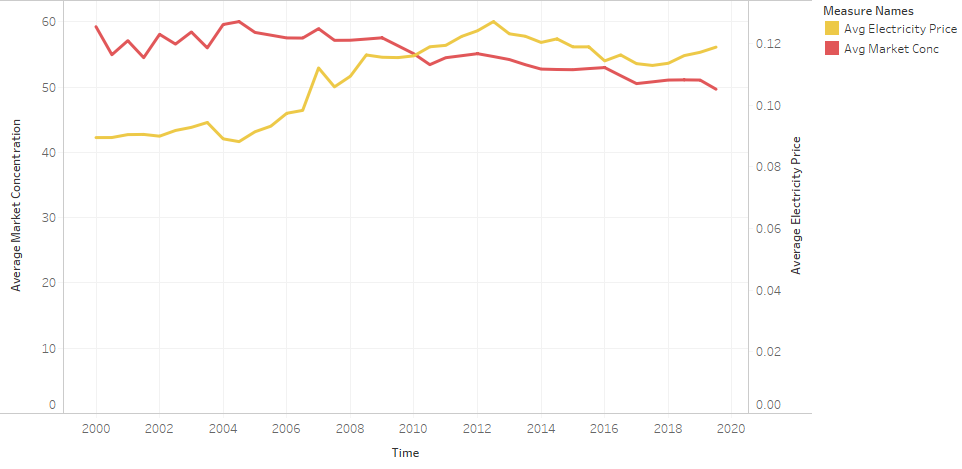
\includegraphics[width=0.9\textwidth]{Images/conc.png}
\caption{Average of biggest supplier share in the market plot against average electricity price. }
\end{center}
\end{figure}
\bigskip

In any case, \textit{Figure 2} also demonstrates how, although the liberalization process has led to the disintegration of national monopolies, it did not lead to a disruptive fall in concentration within the sector. With an average value of the biggest  supplier market share of 50\% the European situation is quite far from the internal market and open competition. There still exist different national and regional markets with the presence of incumbents as main actors in each electricity market. Despite liberalization, the level of concentration is hence quite high.  In \textit{Figure 3}, the focus is on the biggest European markets over the last 20 years: Germany, Spain, France and Italy. It is interesting how notice how they all experienced a slight decrease in market concentration, but with France starting from a concentration value that stands out with respect to the others, with the most important supplier having a market share of 90\%.

\bigskip
\begin{figure}[H]
\begin{center}
\captionsetup{justification=centering}
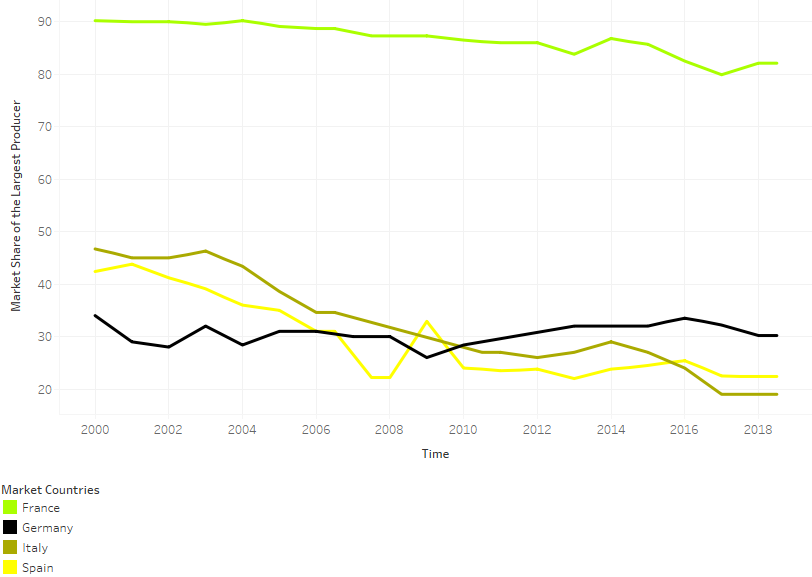
\includegraphics[width=0.9\textwidth]{Images/conc-mc.png}
\caption{Average of biggest supplier share in the market plot for Germany, Spain, France and Italy. }
\end{center}
\end{figure}
\bigskip

One final note of caution: in this section the market share of the biggest supplier in the market was used as a proxy for market liberalization. The higher the share, the more the market is concentrated. However, looking at the largest supplier is a bit limiting and it is used only because data are available from Eurostat. A market in which only two suppliers share the whole market is completely different from one in which the biggest supplier controls half of the market and the rest of it is controlled by very little providers. Yet, the largest supplier market share variable value would be the same.
 
\subsection*{Inflation}

The average increase in prices in a given country is an obvious cause for electricity price surge.

\chapter*{Methodology \& Results}
\section*{Static Model}
\section*{Dynamic Model}

\bibliography{references}{}
\bibliographystyle{plain}

\end{document}